\documentclass{article}
\usepackage{amssymb}
\usepackage{changepage}
\usepackage[fleqn]{amsmath}
\usepackage{cancel}
\usepackage{graphicx}
\title{Gravitational Potential Energy}
\author{SPH-4UI - Tristan Simpson}

\begin{document}
\maketitle

\section{Calculations}
\begin{adjustwidth}{0.5cm}{0pt}
    \textbf{\textit{Formula:}} $E_{g} = -\left(\frac{G \times m_{a}m_{b}}{r_{ab}}\right)$ \\\\
    \textbf{\textit{Constant:}} $G = 6.67 \times 10^{-11}$ $\frac{Jm}{kg^2}$ \\\\
    \textbf{\textit{Diagram:}} \\
    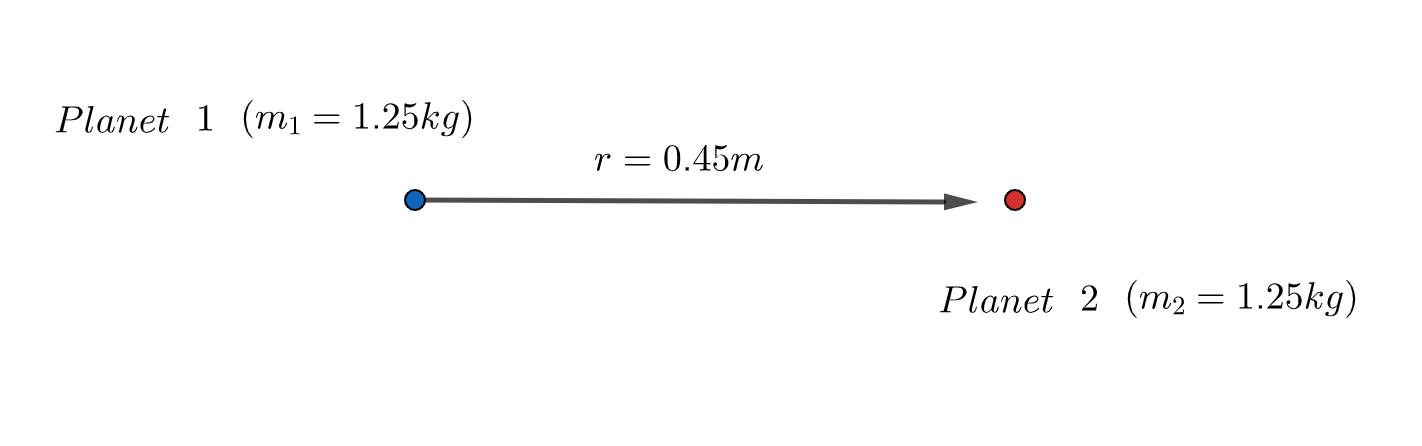
\includegraphics[scale=0.5]{./images/diagram1} \\
    \textbf{\textit{Solve:}} \\
    \begin{flalign*}
        E_{g} & = -\left(\frac{G\times m_{1}  \times m_{2}}{r}\right)          \\\\
              & = -\left(\frac{(6.67\times 10^{-11})(1.25)(1.25)}{0.45}\right) \\\\
              & \approx -2.32\times 10^{-10 }J
    \end{flalign*} \\\\\\\\\\
\end{adjustwidth}

\section{Escape Velocity from Earth}
\begin{adjustwidth}{0.5cm}{0pt}
    \textbf{\textit{Diagram:}} \\
    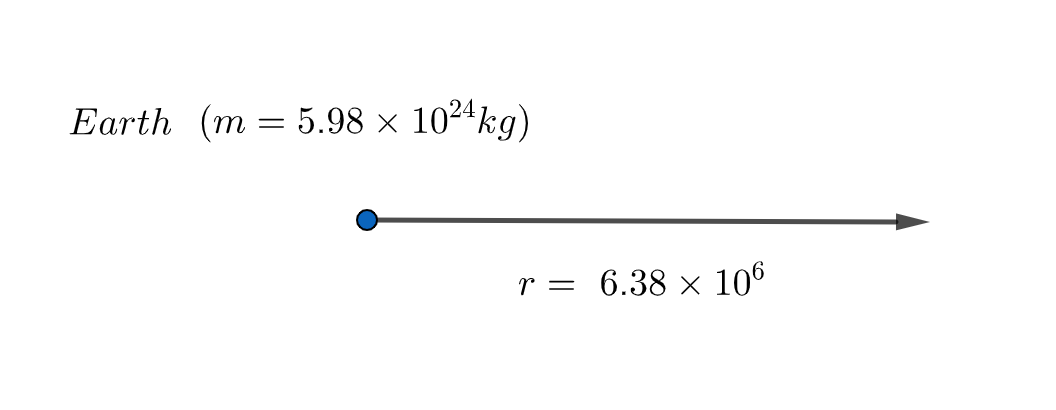
\includegraphics[scale=0.5]{./images/diagram2} \\
    \textbf{\textit{Solve:}} \\
    \begin{adjustwidth}{0.5cm}{0pt}
        \noindent$ E_{tot} = E_{tot}\prime$ \\\\
        $E_{g} + E_{k} = \cancelto{0}{E_{g}\prime} + \cancelto{0}{E_{k}\prime}$   \\\\\\
        $-\left(\frac{G\times m_{shuttle}\times m_{earth}}{r}\right) + \frac{1}{2}m_{shuttle}v^2 = 0$ \\\\\\
    \end{adjustwidth}
    \begin{flalign*}
        \therefore V & = \sqrt[]{\frac{2(G\times m_{shuttle}\times m_{earth})}{rm_{shuttle}}}            \\\\
                     & = \sqrt[]{\frac{2(G\times m_{earth})}{r}}                                         \\\\
                     & = \sqrt[]{\frac{2((6.67\times 10^{-11})(5.98\times 10^{24}))}{(6.38\times 10^6)}} \\\\
                     & \approx 11.2 \frac{km}{s}
    \end{flalign*}
\end{adjustwidth}

\end{document}